\documentclass[aspectratio=169, table]{beamer}
\usepackage[utf8]{inputenc}
\usepackage{listings} 
\usepackage[strings]{underscore}
\usepackage{caption}

\makeatletter
\def\input@path{{../../themes/Pradita}}
\makeatother

\usetheme{Pradita}

\subtitle{IF120203-Programming Fundamentals}

\title{Chatper-01:\\\LARGE{Pendahuluan: Sejarah, Instalasi,\\Hello World}}
\date[Serial]{\scriptsize {PRU/SPMI/FR-BM-18/0222}}
\author[Pradita]{\small{\textbf{Alfa Yohannis}}}


% Define Python language style for listings
\lstdefinestyle{PythonStyle}{
language=Python,
basicstyle=\ttfamily\footnotesize,
keywordstyle=\color{blue},
commentstyle=\color{gray},
stringstyle=\color{red},
breaklines=true,
showstringspaces=false,
tabsize=2,
captionpos=b,
numbers=left,
numberstyle=\tiny\color{gray},
comment=[l]{//},
morecomment=[s]{/*}{*/},
commentstyle=\color{gray}\ttfamily,
string=[s]{'}{'},
morestring=[s]{"}{"},
}

\begin{document}

\frame{\titlepage}

% Add table of contents slide
\begin{frame}[fragile]{Contents}
\vspace{15pt}
\begin{columns}[t]
\begin{column}{.5\textwidth}
\tableofcontents[sections={1-4}]
\end{column}
\begin{column}{.5\textwidth}
\tableofcontents[sections={5-9}]
\end{column}
\end{columns}
\end{frame}

\section{Sejarah}
\begin{frame}{Sejarah Komputer}
	\begin{itemize}
		\item \textbf{Charles Babbage} - Mesin Analitik: Dikenal sebagai bapak komputer, Babbage merancang mesin analitik pada abad ke-19 yang merupakan konsep awal komputer modern.
		\item \textbf{Ada Lovelace} - Program Pertama: Menulis algoritma untuk mesin analitik Babbage, dianggap sebagai programmer komputer pertama.
		\item \textbf{ENIAC (Electronic Numerical Integrator and Computer)} - 1945: Salah satu komputer elektronik pertama yang digunakan untuk perhitungan matematis kompleks.
		\item \textbf{UNIVAC I (Universal Automatic Computer)} - 1951: Komputer komersial pertama yang dirancang untuk keperluan bisnis.
	\end{itemize}
\end{frame}

\begin{frame}{Generasi Komputer}
		\begin{itemize}
			\item \textbf{Generasi Pertama (1940-an - 1950-an):} Menggunakan tabung vakum, seperti ENIAC.
			\item \textbf{Generasi Kedua (1950-an - 1960-an):} Menggunakan transistor, yang lebih kecil dan lebih efisien daripada tabung vakum.
			\item \textbf{Generasi Ketiga (1960-an - 1970-an):} Menggunakan sirkuit terpadu (IC), memungkinkan komputer menjadi lebih kecil dan lebih murah.
			\item \textbf{Generasi Keempat (1970-an - sekarang):} Menggunakan mikroprosesor, yang memungkinkan komputer pribadi dan laptop.
			\item \textbf{Generasi Kelima (Saat ini):} Komputer berbasis kecerdasan buatan (AI) dan teknologi komputasi kuantum.
		\end{itemize}
\end{frame}

\begin{frame}{Kaitan Komputer dan Pemrograman}
	\begin{itemize}
		\item \textbf{Komputer:} Perangkat elektronik yang memproses data dan menjalankan instruksi. Memerlukan perangkat lunak (software) untuk berfungsi.
		\item \textbf{Pemrograman:} Proses menulis kode untuk memberi instruksi kepada komputer. Tanpa pemrograman, komputer tidak dapat berfungsi.
		\item \textbf{Peran Pemrograman:}
		\begin{itemize}
			\item Mengontrol perangkat keras dan menyelesaikan tugas.
			\item Mengembangkan aplikasi untuk berbagai kebutuhan pengguna.
		\end{itemize}
		\item \textbf{Bahasa Pemrograman:} Bahasa yang digunakan untuk menulis kode, seperti Java, C++, dan Python.
	\end{itemize}
\end{frame}


\begin{frame}[fragile]{Sejarah Pemrograman dan Python}
\begin{itemize}
\item Pemrograman komputer dimulai pada abad ke-19 dengan mesin analitik oleh Charles Babbage dan program pertama oleh Ada Lovelace.
\item Bahasa pemrograman awal: Fortran, COBOL, Lisp (1950-an).
\item Bahasa seperti C, Pascal, dan Basic diperkenalkan pada 1970-an dan 1980-an.
\item Bahasa modern seperti Python, JavaScript, dan Rust digunakan dalam berbagai aplikasi.
\item Python: Dikembangkan oleh Guido van Rossum (1991), terkenal dengan sintaks yang sederhana, mudah dibaca, dan komunitas yang besar.
\end{itemize}
\end{frame}

\section{Cara Kerja Python}
\begin{frame}{Python sebagai Bahasa Interpreter}
\begin{itemize}
\item Python bukan \textit{compiled language} seperti C, C++, atau Java, melainkan \textit{interpreted language}.
\item Program Python dieksekusi baris demi baris oleh \textbf{Python Interpreter}.
\item Keuntungan:
	\begin{itemize}
	\item Mudah digunakan dan fleksibel.
	\item Cocok untuk prototyping.
	\end{itemize}
\item Kekurangan:
	\begin{itemize}
	\item Lebih lambat dibanding bahasa yang di-compile.
	\end{itemize}
\end{itemize}
\end{frame}

\section{Compiler vs Interpreter}
\begin{frame}{Compiler vs Interpreter}
\begin{figure}[h]
	\centering
	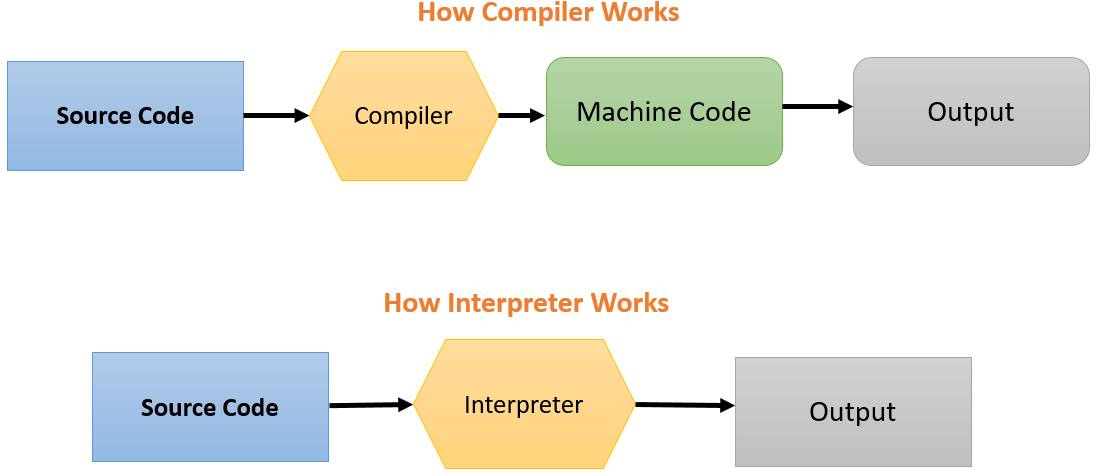
\includegraphics[width=0.7\textwidth]{../../../shared_assets/images/compiler_vs_interpreter.png}
	\caption*{\textbf{Gambar 1:} Perbedaan antara Compiler dan Interpreter}
	\smallskip
    {\tiny Sumber: \url{https://www.ankitweblogic.com/c/compiler-and-interpreter.php}}
\end{figure}
\end{frame}

\section{Instalasi}
\begin{frame}[fragile]{Instalasi di Windows}
\begin{enumerate}
\item Unduh installer Python terbaru dari situs resmi \href{https://www.python.org/downloads/}{python.org}.
\item Jalankan file installer \texttt{.exe} dan ikuti petunjuk untuk menyelesaikan instalasi.
\item Saat instalasi, centang opsi \textbf{``Add Python to PATH''} agar Python otomatis dikenali di Command Prompt.
\item Ikuti petunjuk instalasi hingga selesai.
\item Verifikasi instalasi dengan membuka Command Prompt lalu ketik:
\begin{verbatim}
python --version
pip --version
\end{verbatim}
\end{enumerate}
\end{frame}

\begin{frame}[fragile]{Instalasi di macOS}
\begin{enumerate}
\item Unduh installer Python terbaru dari \href{https://www.python.org/downloads/macos/}{python.org}.
\item Jalankan file installer \texttt{.pkg} dan ikuti petunjuk hingga selesai.
\item Alternatif lain, Anda bisa menggunakan Homebrew dengan menjalankan perintah berikut di Terminal:
\begin{verbatim}
brew install python
\end{verbatim}
\item Setelah instalasi selesai, verifikasi dengan perintah:
\begin{verbatim}
python3 --version
pip3 --version
\end{verbatim}
\end{enumerate}
\end{frame}

\begin{frame}[fragile]{Instalasi di Linux}
\begin{enumerate}
\item Buka terminal dan jalankan perintah berikut untuk memastikan repositori diperbarui dan Python terpasang:
\begin{verbatim}
sudo apt update
sudo apt install python3 python3-pip
\end{verbatim}
\item Verifikasi instalasi dengan perintah:
\begin{verbatim}
python3 --version
pip3 --version
\end{verbatim}
\end{enumerate}
\end{frame}

\section{IDE}
\begin{frame}[fragile]{Apa Itu IDE?}
\begin{itemize}
\item Integrated Development Environment (IDE) menyediakan fasilitas lengkap untuk pengembangan perangkat lunak.
\item Umumnya mencakup editor kode, kompiler/interpreter, debugger, dan alat manajemen proyek.
\item IDE mempermudah pengembangan dengan antarmuka yang terintegrasi.
\end{itemize}
\end{frame}

\begin{frame}[fragile]{Cara Menginstal Visual Studio Code}
\begin{enumerate}
\item Unduh installer VS Code dari situs resmi \url{https://code.visualstudio.com/}.
\item Pilih installer sesuai sistem operasi Anda (Windows, macOS, atau Linux).
\item Jalankan file installer dan ikuti petunjuk instalasi.
\item Setelah instalasi selesai, buka aplikasi VS Code.
\end{enumerate}
\end{frame}

\begin{frame}[fragile]{Cara Membuat Proyek Python Baru di VS Code}
\begin{enumerate}
\item Buka VS Code dan pilih folder kerja (workspace) untuk proyek Python.
\item Buat file baru dengan ekstensi \texttt{.py}, misalnya \texttt{main.py}.
\item Pastikan Python extension sudah terpasang di VS Code.
\item Pilih interpreter Python yang sesuai melalui Command Palette (\texttt{Ctrl+Shift+P} > \texttt{Python: Select Interpreter}).
\item Mulai menulis kode Python di file tersebut.
\end{enumerate}
\end{frame}

\section{Hello World}
\begin{frame}[fragile]{Kode Python: hello_world.py}
\begin{lstlisting}[style=PythonStyle]
print("Hello World")
\end{lstlisting}
\end{frame}

\begin{frame}[fragile]{\LARGE{Panduan Menjalankan Program Python}}
\begin{enumerate}
\item Buka terminal atau command prompt.
\item Navigasikan ke direktori tempat file \texttt{hello_world.py} disimpan (Default direktori jika membuka terminal dari VS Code adalah direktori proyek saat ini). 
\item Jalankan perintah \texttt{python hello_world.py}.
\end{enumerate}
\end{frame}

\begin{frame}[fragile]{Kode Python: hello_world_with_input.py}
\begin{lstlisting}[style=PythonStyle]
nama = input("Masukkan nama Anda: ") # Menerima input dari pengguna

print("Hello " + nama + "!") # Menampilkan output dengan input pengguna
\end{lstlisting}
\end{frame}

\section{Latihan}
\begin{frame}[fragile]{Latihan 1: Membuat Program Pengenalan Diri}
\begin{itemize}
\item Buat file baru dengan nama \textbf{introduction.py} yang dimana program harus menerima input nama, usia, dan domisili dari pengguna kemudian mencetak pesan dengan format yang ditentukan
\end{itemize}
\end{frame}

\begin{frame}[fragile]{Latihan 1: Kode Program}
\begin{lstlisting}[style=PythonStyle]
nama = input("Masukkan nama Anda: ")
prodi = input("Masukkan program studi Anda: ")
angkatan = input("Masukkan angkatan Anda: ")

print("Halo! Nama saya " + nama + ". Saya mahasiswa program studi " + prodi + " tahun angkatan " + angkatan + ".")
\end{lstlisting}
\end{frame}

\begin{frame}[fragile]{\LARGE{Latihan 2: Memformat teks menggunakan f-string}}
\begin{itemize}
\item Latihan ini bertujuan untuk belajar memformat teks (\textit{string}) menggunakan \textbf{f-string}, membuat output lebih rapi tanpa perlu menggunakan operator \texttt{+} sebagai penghubung antara teks. 
\item Buat file baru dengan nama \textbf{introduction_with_fstring.py} dan isinya mirip dengan, namun format outputnya menggunakan \textbf{f-string}
\end{itemize}
\end{frame}

\begin{frame}[fragile]{Latihan 2: Kode Program}
\begin{lstlisting}[style=PythonStyle]
nama = input("Masukkan nama Anda: ")
prodi = input("Masukkan program studi Anda: ")
angkatan = input("Masukkan angkatan Anda: ")

print(f"Halo! Nama saya {nama}. Saya mahasiswa program studi {prodi} tahun angkatan {angkatan}. Output dihasilkan menggunakan f-string")
\end{lstlisting}
\end{frame}

\begin{frame}[fragile]{Latihan 3: Escape Character}
\begin{itemize}
\item \textit{Escape Character} merupakan karakter khusus yang digunakan (biasanya diawali dengan \texttt{\textbackslash}) yang digunakan di dalam string untuk mengatur penataan teks atau menampilkan karakter spesial.
\item Dengan escape character, kita bisa:

\begin{itemize}
    \item Membuat teks pindah baris: \texttt{\textbackslash n}
    \item Menambahkan tabulasi: \texttt{\textbackslash t}
    \item Menulis tanda kutip di dalam string: \texttt{\textbackslash "}
    \item Menampilkan backslash asli: \texttt{\textbackslash\textbackslash}
\end{itemize}

\end{itemize}
\end{frame}

\begin{frame}[fragile]{Latihan 3: Kode Program}
\begin{lstlisting}[style=PythonStyle, firstnumber=1]
print("Hello\nWorld") # Membuat teks pindah baris
print("Hello\tWorld") # Menambahkan tabulasi
print("Hello \"World") # Menulis tanda kutip di dalam string
print("Hello \\ World") # Menampilkan backslash asli
\end{lstlisting}
\end{frame}

\section{Soal Latihan}

\begin{frame}[fragile]{Soal Latihan}
	Berikut adalah beberapa soal latihan tambahan untuk menguji pemahaman Anda mengenai konsep yang telah dipelajari:
\end{frame}

\begin{frame}{Soal 1}
	Buat program bernama \texttt{biodata.py} yang meminta input berupa:
	\begin{itemize}
		\item Nama lengkap
		\item Umur
		\item Hobi
	\end{itemize}
	Cetak output dengan format berikut menggunakan \textbf{f-string}. Berikut merupakan contoh input dan output yang diharapkan:
\end{frame}

\begin{frame}[fragile]{Soal 1}
	\begin{verbatim}
	Input:
	Masukkan Nama Lengkap: Jane Hopkins
	Masukkan Usia Anda: 20
	Masukkan Hobi Anda: Ngoding

	Output:
	Halo, nama saya Jane Hopkins. Saya berusia 20 tahun dan hobi saya 
	adalah Ngoding.
	\end{verbatim}
\end{frame}

\begin{frame}[fragile]{Soal 2}
	Buat program bernama \texttt{quote.py} yang menampilkan kutipan favoritmu. Gunakan \textbf{escape character} untuk menampilkan tanda kutip di dalam string. Contoh output:

	\begin{verbatim}
	Input:
	Masukkan kutipan favoritmu dari Albert Einstein: "Imagination 
	is more important than knowledge."

	Output:
	Kata Albert Einstein: "Imagination is more important than knowledge."
	\end{verbatim}
\end{frame}

\begin{frame}{Soal 3}
	Buat program bernama \texttt{schedule.py} yang menampilkan jadwal kuliah. Gunakan \textbf{tabulasi} (\texttt{\textbackslash t}) untuk merapikan kolom. Contoh output:
	\\[15pt]
	\begin{tabular}{l l l}
		\textbf{Hari} & \textbf{Waktu} & \textbf{Mata Kuliah} \\
		Senin & 07.00 & Algoritma \\
		Selasa & 09.00 & Basis Data \\
		Selasa & 13.00 & Pemrograman Dasar \\
	\end{tabular}
\end{frame}

\section{Penutup}
\begin{frame}[fragile]{Penutup}
\begin{itemize}
\item Sejarah pemrograman, cara instalasi Python dan Visual Studio Code, dan pengenalan dasar Python.
\item Latihan-latihan untuk memberikan pengalaman pengenalan Python.
\end{itemize}
\end{frame}

\end{document}
